\section{波动力学}


\subsection{波粒二像性}


我们对粒子和波动的概念来自直接的经验。和粒子有关的经验对象:小到石子大到天上的星星等;和波动有关的经验对象:最常见的例子是水波,还有拨动的琴弦等。但这些还不是物理中所说的模型,物理中所谓粒子和波动是理想化的模型,是我们头脑中抽象的对象。


\subsubsection{粒子的图像}


在经典物理中,粒子的概念可进一步抽象为:大小可忽略不计的具有质量的对象,即所谓质点。质量(mass)在这里是新概念,mass的原初含义就是多少,这里引申为对物体惯性质量多少的量度。一个西瓜,比西瓜籽的质量大,因为西瓜里包含的物质比西瓜籽多,西瓜保持自身运动状态的能力比西瓜籽强。

为叙述的简单,我们现在可把粒子等同于质点。要描述一个质点的运动状态,我们需要知道其位置$x$和速度$v$,速度是对位置的微分。

\begin{equation}
v = \frac{d x}{d t}
\end{equation}

这是莱布尼茨的记号,我们有时也把它记为$\dot x$,$\dot x$是牛顿的记号。记号会有助于我们思维,比如$\dot x$比较简短,而$frac{d x}{d t}$则会提醒我们微分运算的结构,即微分是如何定义的,粒子在时间$\Delta t$内飞行了$\Delta x$,然后我们对$\Delta t$取极限。

而取极限是构造这样一个可以count的过程,(1)首先,$\Delta t = 1$秒;(2)$\Delta t = 0.1$秒;(3)$\Delta t = 0.01$秒;(4)……。假设运算$\frac{\Delta x }{\Delta t}$在这样一个可以count的过程里趋于一个确定的数,我们就说极限存在。

我们研究数学是为了应用于物理的研究,而物理研究的对象都是确定的现象,这决定了我们特别对这类数学形式感兴趣,比如在这里就是极限存在,如果极限不存在,我们也要努力调整数学结构使其存在,否则我们正在使用的数学对物理研究就是不趁手的。

对时间做微分就必须讨论时间,时间也是一个直观的概念,这里我们可把时间描述为一个时钟,我们会发现当指针指到不同位置时,质点的位置可能不同,于是指针的位置就定义了时刻$t$。有了时刻$t$,我们对质点的描述就变成了$x(t)$,在想象中动起来的质点就是一条线,就是轨迹。由$x(t)$可定义速度$v(t)$,考虑到质点还有质量$m$,我们现在用位置$x$和动量$p$这一对量来表示质点的运动状态。

$x$和$p$并放$(x, p)$就是相空间(phase space)中的一个点。相空间是抽象的数学空间,比如在这里我们要描述一个粒子的运动,位置是三维的($x, y, z$),动量也是三维的($p_x, p_y, p_z$),相空间就是六维的。我们用六维超空间中的一个点来描述一个质点的运动。

在日常经验中我们还有相互作用或所谓力的概念,我们在地球上拎起不同质量物体时肌肉的紧张程度是不同的,或者说在地球上用弹簧秤拎起不同质量物体时弹簧的拉伸程度是不同的。

以上我们对质量、时间、力等的定义都是直观的,是可以操作的。按照以上思路进行研究,研究落体的运动,研究天体的运动,……最终诞生了牛顿的经典力学。这里我们可简单地用两个公式:$F=ma$(牛顿第二定律)
和$F = \frac{GMm}{r^2}$(万有引力公式)
来代表牛顿力学。前者是质点的运动方程,用数学的语言说是一个关于位置$x$的二阶微分方程,根据微分方程的理论,只需要知道初始时刻$t=0$时的位置$x$和速度$v$即可求出以后任意时刻$t$质点所处的位置,即轨迹$x(t)$。

需要强调的是一旦我们知道$t=0$时$x$和$v$的精确值(没任何误差),$x(t)$的取值也是精确的,即我们得到的是对质点未来演化的精确预测,并且这个求解对$t < 0$也精确成立,这意味着我们还可精确地反演质点的历史。这些结论是由牛顿力学的数学结构严格保证的,即轨迹是一根理想的线,它没有宽度。

现在我们就有了一个关于世界的整体图像:宇宙是由很多质点构成的复杂系统,它们两两之间的相互作用由$F=\frac{GMm}{x^2}$决定,对每一个质点我们又可列出$\sum\limits_i F_i = ma$这样的运动方程,$\sum\limits_i
F_i$表示质点所受的合力,与其他质点的位置有关,因此这是一个联立的二阶微分方程组。

还是根据数学的理论,如果我们知道了初始时刻$t=0$时每个质点的位置和速度,我们即可无限精确地知道系统内每个粒子的轨迹。这在哲学上被引申为所谓的“决定论”,我们会倾向于相信:世界只不过是个巨大的机械,人生的命运是确定的,事物的演化也是确定的等等。

当然要想在某一时刻同时测量出全世界所有粒子的位置和速度是不可能的,但这是否意味着——“某一时刻全世界所有粒子具有确定的位置和速度”——本身就不存在呢?有些人可能会持怀疑的态度。另一些人会倾向于相信,当然这种相信并无充分的证据,相信的好处是我们可建立起一个关于世界的整体图像,整个世界变得有秩序了,可以理解了。

不管我们是否相信决定论,牛顿力学本身获得了巨大成功,解释了大到行星运动,小到苹果落地等广泛的现象,因此主流物理学家在100多年前相信牛顿力学提供了描述整个世界的基础。

\subsubsection{波动的图像}

在有了粒子的图像后,我们很容易把波动还原为很多粒子的集体运动。比如最简单的波动,抖动绳子可产生一维波。要解释这样的波动现象,最简单的模型就是假想把绳子分成很多很多份,每部分很小以至我们可将其视为质点,质点间的力用弹性力表示。看起来这就是一根弹簧,上面放了很多等质量的小球,如果你横向摇晃第一个小球,这种运动就会渐次地传递给其他小球,像墨西哥人浪一样,波行进的方向和小球偏离的方向垂直,即所谓横波;如果你纵向压缩拉伸第一个小球,这种纵向的振动也会渐次地传递给其他小球,即所谓纵波,纵波的例子是声波。

由此可见波动是一种整体运动,是由很多粒子参与步调统一的运动。最简单的波动是单色平面波,即体现为正弦或余弦函数:$A\cos(kx - \omega t)$。波动的特点是会传播出去,因此你很难说波在什么地方,或说了也没啥意义,因为它无所不在。对单色平面波来说,波动在每一点的状况都是一样的,但我们可以发现相邻波峰间距离总是相同的,于是可定义波长:$\lambda$,我们还发现每个质点振动一个周期的时间也是相同的,因此可定义频率:$\nu$。

很多质点的整体运动——“波动”——和“粒子”是很不同的,描述粒子的运动,使用位置和动量,描述波动使用振幅$A$、波长$\lambda$和频率$\nu$。粒子的特点是分立的,每个粒子会集中地携带能量$E$和动量$p$,而波动的特点则是弥散的,能量会均匀地分布在介质(中的每个质点)上,波动的能量密度正比于振幅的平方($A^2$)。

粒子是分立的,它们各自在虚空中运行,互相用引力勾连着;而波动是连续的、充盈的整体运动,由波动方程描述。从这个意义上我们说粒子的图像和波动的图像是排斥的,即我们无法想象一个对象既是粒子又是波动。

\subsubsection{电磁波}

尽管粒子的图像和波动的图像是互相排斥的,我们仍会认为粒子的图像更本质,波动的图像可还原为粒子的语言,因此是从属的。但物理学家很快又发现了一种新的波——电磁波。

电磁现象是不同于机械力学(即上面讨论的质点或质点系的运动)的新现象。麦克斯韦是电磁学中的牛顿,他提出的麦克斯韦方程组是解释电磁现象的基础。利用麦克斯韦方程组最重要的预言是“光波就是电磁波”或“电磁波就是光波”。

所谓电磁波就是电场($E$)和磁场($B$)在空间中的传播,和机械波中质点振动会在空间中传播一样,它们都满足类似的波动方程,只是波动传播的速度不同而已。

物理学家自然提出一个任务,即能否把电磁波还原为纯粹的机械运动?追求统一的物理是物理学家永恒的追求,牛顿使天上的物理(行星运动)和地上的物理(苹果落地)统一,麦克斯韦使光学和电磁学统一,那么经典力学和经典电磁学也应该是统一的。但实际上把电磁波还原为机械运动的努力一直没取得啥进展。

如果考虑到光波或电磁波无法还原为机械运动,我们现在可说粒子的图像和波动的图像在概念上是同等重要的,但在量子场论中,粒子被解释为场的激发,这有点把粒子还原为场的意思。

\subsection{双缝实验}

量子力学诞生于原子物理学,即关于原子尺寸物理现象的研究。今天我们知道原子大约是0.1纳米,而人类肉眼可分辨(假设可借助光学显微镜)的尺寸大约是可见光波长的数量级——几百纳米,即我们研究的对象小了至少几万倍。从这个意义上说量子现象是超越于我们日常经验之外的。当我们提到粒子和波动的时候,即便没有系统地学习过物理学,我们也可借助日常经验在“望文生义”的意味下知道粒子大致指的是什么现象,波动指的是什么现象。但当我们讲到原子或电子的运动时,我们就没有这样的直观了。

~

所以如果不系统地补足物理学史上关于原子物理的研究的话,就必须得有一个机会供我们直观地体验一下量子现象。费曼曾提出著名的双缝实验\footnote{费曼提出单粒子双缝实验时并未真的试图实现它,但随着技术的进步现在已有物理学家完成真正的单电子双缝干涉实验:\url{http://physicsworld.com/cws/article/print/9745}},通过这个实验我们可建立量子力学的基本概念——波粒二像性。

在光学中也有双缝实验,光通过双缝,绕过障碍物,互相叠加,最终在屏上呈现出明暗相间的条纹状分布,这个被称为干涉。干涉现象很容易用波动的图像解释:光是电磁波,当波照射到双缝上时,每个缝相当于是新的波源(惠更斯原理),每个波源都会发出一系列波峰和波谷,当两个波峰相遇时则加强呈现出明亮的条纹,当一个波峰和一个波谷相遇时则抵消呈现出暗条纹。

\begin{figure}[htbp]
\begin{center}
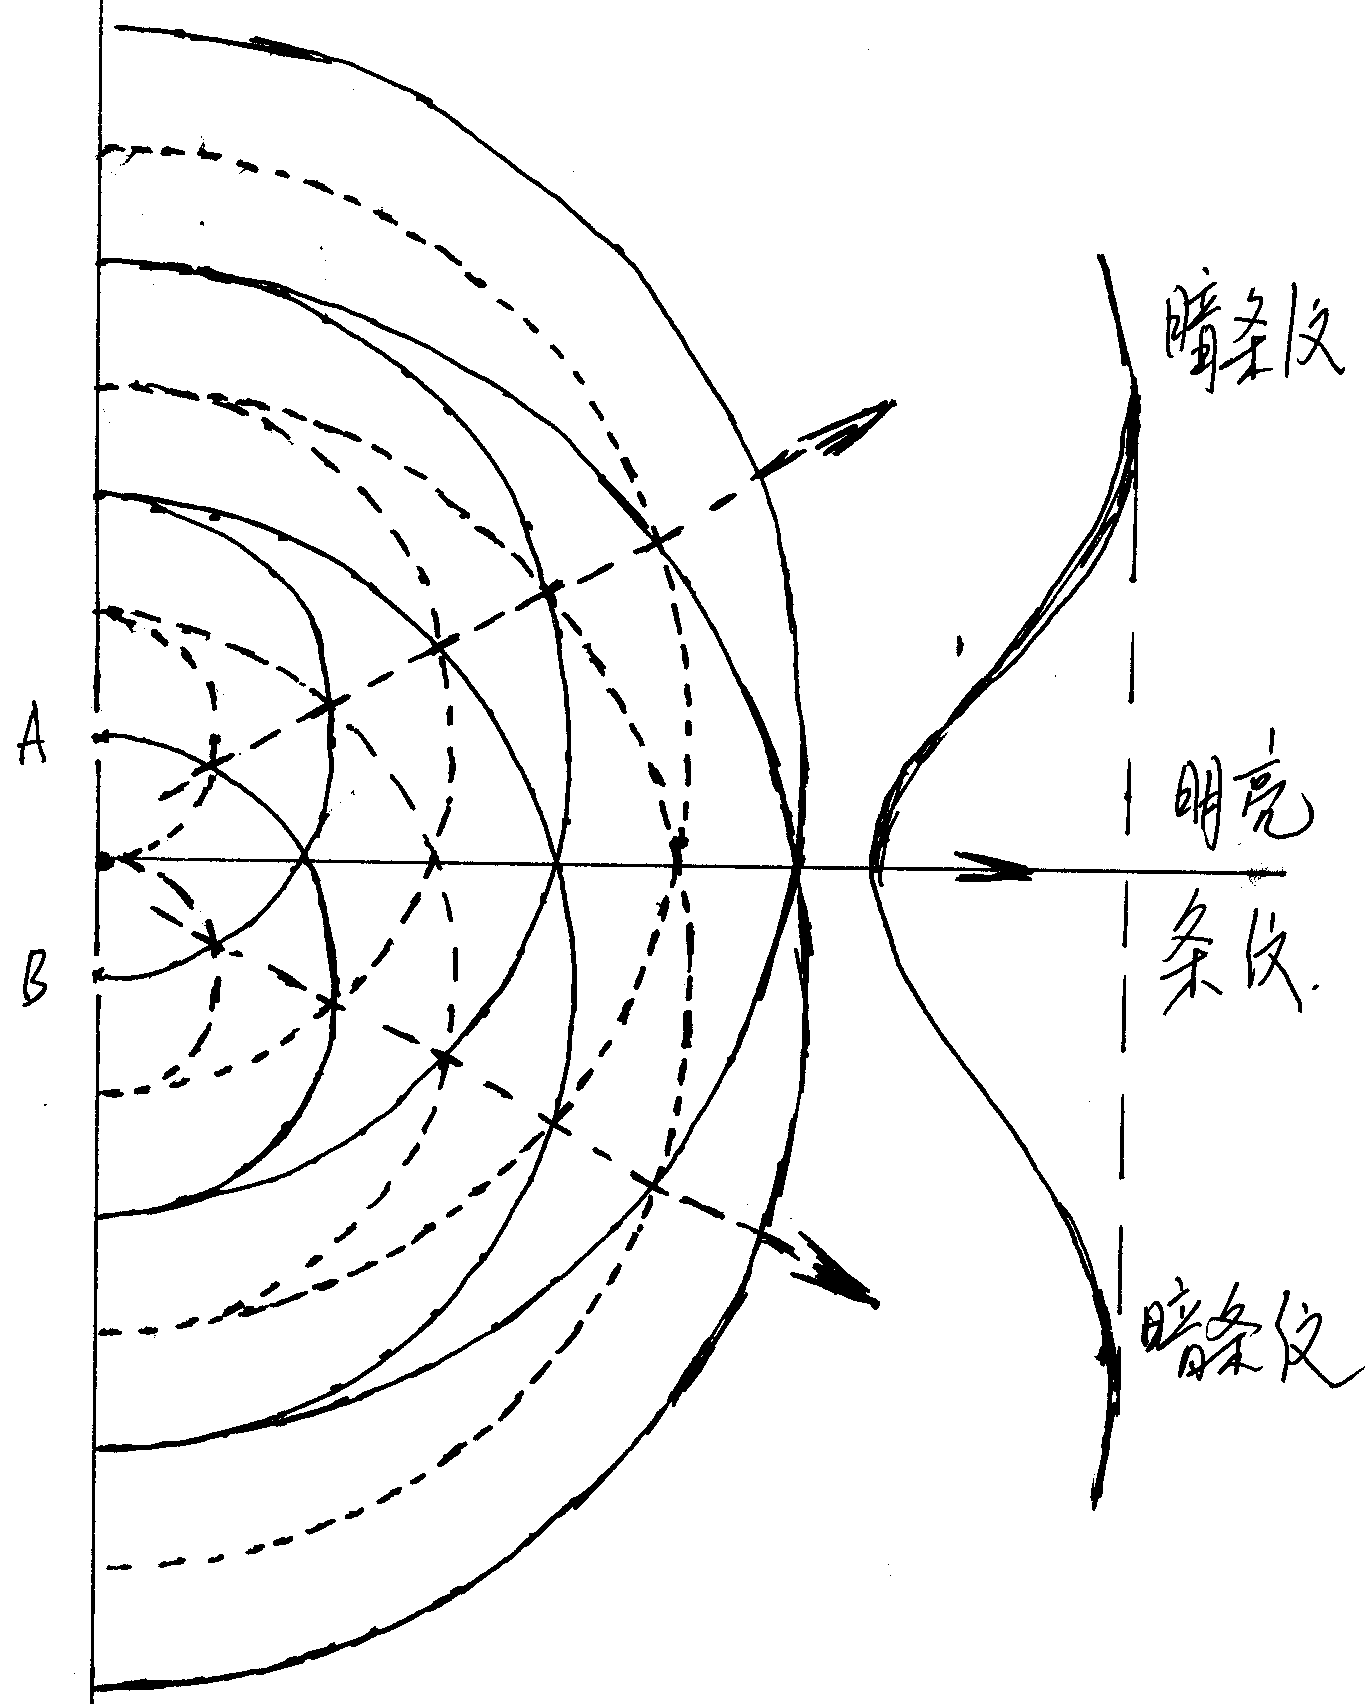
\includegraphics[width=10cm]{QuantumIntro/doubleslit.png}
\caption{双缝干涉示意。}
%\label{default}
\end{center}
\end{figure}

现在我们假设以一束电子入射到双缝上,看看会发生什么现象。电子是量子力学对象,但现在我们先猜测它就是经典的粒子,这种情形下电子穿过双缝——呈上、下两个条状分布。费曼讲的是机枪扫射,看子弹如何穿过双缝,根据日常经验子弹无法绕过障碍,将集中地分布在双缝的方向上。

那么实验的结果是什么呢?是明、暗相间的条纹状分布,就好像光学中的双缝实验结果一样。这是否意味着电子是一种波动呢?就像迄今为止我们都理所当然地认为光就是一种波动,一种电磁波。

我们可以再做实验,让电子一个、一个地通过双缝,看看是否会有干涉现象。实验结果是电子将随机地出现在任意位置,我们根本无法预测电子下一次出现在什么位置。但我们也注意到电子并未弥散开来,每次都只出现在一个位置,这说明电子还是粒子。另外一个特点是当我们进行很多次这样的单电子双缝干涉实验后,电子的总体分布会趋于明暗相间的干涉条纹。

有趣的是,对于我们一直认为是波动的“光”,我们也可完成类似的实验,即当我们降低光的强度,最终我们发现光竟然也是由一个一个的粒子——“光子”组成的。当光强极弱时,我们可完成所谓“单光子干涉实验”,单光子穿过双缝对应一个随机的位置,很多单光子事件累积起来呈现干涉条纹。实际上人眼就是理想的“单光子”探测器,生理实验表明只需要5个光子就可使视杆细胞兴奋。

因此,把电子(或光子)简单地设想为经典的粒子或经典的波动都是不可能的,现在我们说电子(或光子)首先是粒子,但它不是经典的,它的运动状态不能用位置$x(t)$和动量$p(t)$描述,而需要用波函数$\psi(x,t)$来描述。这就是所谓波粒二像性,这与日常经验中的粒子是两回事,但物理学家们一般还称呼它们是粒子。

\subsection{波函数}

根据量子力学,粒子的运动状态是由波函数来描述的,其实经典的波动也是由波函数来描述的。量子力学中的波
函数和经典波动波函数的区别在于:经典波动波函数有确切的物理含义,比如电磁波波函数表示的是变化的电场或磁场;量子力学中波函数不对应确切的物理含义,
它一般是复函数,而物理量(如位置、动量)的取值是实数,但物理系统中所有信息却又都包含在波函数中,即根据波函数我们可求出物理量的取值。从数学形式上
看波函数很类似经典波动的波函数,因为经典波动为计算方便也常常表示为复函数的形式;而量子力学中波函数在某些特定情况下也可表示为实函数的形式。这给思考量子力学问题带来很多直观上的好处,因为想象一个经典波动总是很容易的。

最简单的波函数是单色平面波(plane wave):

\begin{equation}
\psi_k (x, t) = A e^{i(kx -\omega t)}
\end{equation}

它所描述粒子的动量是:$p = \hbar k$,能量是:$E = \hbar
\omega$(前者是德布罗意的贡献,后者是普朗克的贡献)。动量的表达式很有用,稍作变形:

\begin{equation}
\lambda = \frac{h}{p}
\end{equation}

这个公式代表了波动语言(左边)和粒子语言(右边)的“翻译”关系。

如前所述,波函数本身——是个复数——没有物理意义,但其绝对值的平方——$\psi^* \psi $是个实数——代表发现粒子的几率密度,这叫做波函数的统计解释(或玻恩解释)。

如果要使得波函数的模方$\psi^*(x) \psi(x)$就是几率密度$\rho(x)$,我们就必须把波函数归一化(Normalization),使得:

\begin{equation}
\int \psi^* \psi dx =1
\end{equation}

粒子的平均位置是:

\begin{center}
粒子的位置 $\times$ 粒子在某处的几率
\end{center}

表示为数学的式子:

\begin{equation}
\overline{x} = \int x | \psi(x) |^2 dx = \int \psi^*  x \psi  d x
\end{equation}

量子力学中还有一条基本原理——“态的叠加原理”(或波函数的叠加原理):

\begin{quote}
如果$\psi_1$代表物理系统一个可能的态,$\psi_2$代表另一个可能的态,那么$c_1\psi_1 + c_2\psi_2$也是一个可能的态。(这里$c_1$,$c_2$是任意复数)
\end{quote}

利用“波函数的统计解释”和“态的叠加原理”,可以很容易理解费曼双缝实验,单电子通过双缝,可用如下波函数表示:

\begin{equation}
\psi  = \psi_1 +  \psi_2
\end{equation}

这里的1和2并不是表示1、2两个电子,单电子意味着只有一个电子,$\psi_1$和$\psi_2$都是这个电子波函数的一部分,1 对应的是上缝,2对应的是下缝。电子的几率分布为:

\begin{equation}
\left( \psi_1^* + \psi_2^*  \right) \left( \psi_1 + \psi_2  \right) = |\psi_1|^2 + |\psi_2|^2 + \psi_1^*\psi_2 +
\psi_1\psi_2^*
\end{equation}

这相当于经典光学中两束光波的迭加,体现为明暗相间的条纹,从数学上说它是由干涉项$\psi_1^*\psi_2 + \psi_1\psi_2^*$导致的。

假设:$\psi_1 = |\psi_1| e^{i \theta_1}$,$\psi_2 = |\psi_2| e^{i \theta_2}$, 则:

\begin{equation}
\psi_1^* \psi_2 + \psi_1 \psi_2^*  = 2 |\psi_1 | \cdot | \psi_2 | \cos (\theta_1 -\theta_2)
\end{equation}


\subsubsection{测量}


我们继续对最简单的波函数:$A e^{i(kx - \omega t)}
$做一些讨论,假设我们设法测量一下粒子的位置$x$
\footnote{利用超快光学测量电子运动的最新进展:\url{http://focus.aps.org/story/v21/st7}
这里是通过制备很多相同电子波函数,然后测量不同阶段电子的位置来获得电子运动图像的,并非是对相同电子运动的持续测量。}。

根据统计解释,波函数绝对值的平方是粒子的分布几率,由于波函数的振幅是常数,粒子是等几率分布的,因此我们可能在空间中任意地方等几率地观测到粒子。那么对于一次具体的测量,粒子将出现在何位置?我们没法预测,只知道会在空间任何地方。

暂不讨论我们是如何测量粒子位置的,假设$t=0$时我们完成了一次成功的测量,我们会观测到粒子在某确定位置$x=x_0$
,现在我们问:在$t=0$之前的一瞬间粒子在什么地方?关于这个问题有两种答案\footnote{关于波函数统计解释和波函数坍缩更详尽的讨论可参考:D. J. Griffiths, Introduction to Quantum Mechanics, pp2-5;}:

\begin{figure}[htbp]
\begin{center}
\includegraphics[width=8cm]{QuantumIntro/peak_atx0.ps}
\caption{假设$t=0$完成一次成功的测量,测得粒子在$x=x_0$附近;}
%\label{default}
\end{center}
\end{figure}


\begin{enumerate}
\item 

虽然我们无法精确地知道粒子在什么地方,但我们可推测其一定在$x_0$附近,因为根据狭义相对论,粒子运动速度存在一上限,因此在测量前一瞬间,粒子应在$x_0$附近。那么在测量前一瞬间,波函数还是单色平面波吗?因为我们考虑的是测量前,在此操作前波函数无任何理由发生变化,因此应当仍然是单色平面波。但根据量子力学统计解释,粒子应等几率地分布在整个空间,而不是仅仅分布在$x_0$的附近。看来根据量子力学无法得到关于粒子的全部信息,从这个角度说量子力学是不完备的。因此一定还存在某种未知因素,决定了粒子以何种方式在$x_0$附近,因为不知道该因素到底是什么,我们就管它叫隐变量(hidden variables)。这是对量子力学的一种态度,即认为量子力学是不完备的,我们需要发展一种新理论取而代之。持这种观点的物理学家有爱因斯坦、玻姆等。

\item

这一派物理学家认为基于波函数和统计解释的量子力学是完备的,我们可称之为正统派,对创建量子力学有直接贡献的玻尔、玻恩、海森堡等都属于这一派。正统派提出“波函数坍缩”来描述量子力学的测量过程。测量前是单色平面波,粒子等几率地处在整个空间,一次成功的测量意味着在这一瞬间,波函数坍缩为一位置在$x_0$附近的尖峰形函数(数学上叫$\delta$函数,$\delta$函数仅在$x_0$取值不为0,其他地方都是0)。根据统计解释,粒子只能在$x_0$位置,自然这是一次成功的测量,因为我们得到了唯一的位置,在$t=0$之后,我们再做测量,也只能获得$x_0$这一确定性的结论,因为尖峰函数再坍缩也只能是尖峰函数。那么正统解释是否意味着与狭义相对论矛盾呢?或者说我们是否可利用波函数坍缩来构造一个可以携带信息的超过光速的信号呢?仔细的分析否定了这种设想,在这里我们暂不展开讨论。对这个问题的深入讨论引发了量子信息这个前沿领域。

\end{enumerate}

这两派意见,到底哪一派正确呢?贝尔后来针对隐变量理论提出了一个不等式——贝尔不等式,如果隐变量理论成立,不等式成立;如果正统解释成立,则不等式可以不成立。但迄今为止的各种实验对隐变量理论都是不利的,或者说量子力学是完备的,波函数中包括了粒子运动的所有信息。

\subsubsection{经典和量子的界限}

物理学家的基本信念是只有一个物理。原来经典物理可以描述的物理现象,比如行星的运动和几何光学也适用于量子力学。原则上量子力学应适用于所有的物理现象,只是对这些问题的处理会比较繁琐而已,而且经过繁琐的计算我们会发现奇异的量子效应被抵消掉了,这解释了为什么我们使用“错误”的经典理论也能得到正确的结果。

此外物理学是非常灵活,具有实用和工具精神的,当我们面对复杂问题时,大胆地舍去次要因素,只考虑主要因素并得到一个简单有效的算法始终是物理学的核心,而这么做的核心是发现看待事物的新角度,即简单有效是基于新形式的发现和新类的发现。严格求解或回答形而上学意义下僵硬的“是”的问题(比如“电子到底是波还是粒子”)从来不是物理学的趣味。

讨论经典和量子的界限\footnote{关于量子和经典的界限,可继续阅读:\url{http://physicsworld.com/cws/article/print/21590}},目的并不是给出经典物理和量子物理分别适用的界限(只有一个物理),而只是在讨论什么时候必须使用量子力学,或什么时候量子效应不可忽略。

我们可以用一个简单的计算来讨论,量子效应比较明显意味着我们必须用波函数描述粒子,意味着干涉效应比较明显。回忆公式:$\lambda = \frac{h}{p}$,左边是描述波动性的波长,如果波动性较明显,说明波长应比较长,比如说达到几百纳米(达到可见光波段)。这意味着等式右边:$h$必须越大越好,$h$是普朗克常数,恰恰是个很小很小的物理量,这解释了为什么我们平时观察不到量子效应。$p$是粒子动量,应越小越好,但再小也有上限,宏观物体普遍存在无规则热运动,无规则热运动能量可使用$E=k_B T$来估计(即温度越高,无规则热运动越激烈,这也与我们的常识吻合)。现在$p= \sqrt{2 m k_B T}$,$k_B$是另一个物理常数——玻尔兹曼常数,

\begin{equation}
k_B = 1.3806488 \times 10^{-23} J/K
\end{equation}

我们可讨论:

\begin{enumerate}
\item 

m越小越好,这解释了为什么我们会在原子系统中观察到量子现象,因为原子足够小;

\item

另一方面$T$(温度)越低越好,这解释了为什么在低温条件下我们会观察到宏观量子现象,比如超导、超流、超固体\footnote{“超级固体”(super solid)是个很新的研究领域,生活大爆炸中的谢耳朵曾提到过。}和玻色凝聚等。

\end{enumerate}

\subsection{薛定谔方程}

根据量子力学,系统状态是由波函数描述的,假设我们知道某时刻系统的波函数$\psi(t_0)$,我们希望知道系统是如何随时间演化的,即知道未来某时刻的波函数$\psi(t)$。波函数随时间演化的规律是由薛定谔方程给出的:

\begin{equation}
i \hbar \frac{\partial \psi}{\partial t} = \hat H \psi
\end{equation}

这里$\hat H$是哈密顿算符。

薛定谔方程可能是物理学中最重要的方程,其地位很类似于牛顿力学中的牛顿第二定律$F=ma$。它们都是描述随时间演化的动力学方程,不同之处在于牛顿第二定律中的加速度是对时间的二阶微商,因此需要知道初始时刻的位置$x_0$和速度$v_0$才可求解,而薛定谔方程中出现的是对时间的一阶微商,因此只需要知道$\psi(t_0)$就可确定$\psi(t)$。牛顿第二定律和薛定谔方程都是确定性的方程,一旦初始条件确定了,未来的演化是唯一确定的,不同的是牛顿力学中求出的是轨迹,而量子力学中求出的是波函数。轨迹代表了可视化的物理运动(比如开普勒的椭圆),而波函数则是一个复函数并不直接对应任何实际物理量。

但我们又说波函数中已经包含了物理系统的所有信息,因此我们关心的物理量(也称观测量或力学量)可通过特定的数学步骤由波函数导出,当然并非所有经典力学中可获得的信息在量子力学中也可获得。比如:我们在量子力学中无法同时获得一个粒子的位置和动量的取值,但在经典力学中我们是可以获得的。

考虑到两种理论内在的数学结构不同,有这样的区别应该也不算太出乎我们的意料吧。

%%%

\subsubsection{算符}

考虑最简单的波函数——单色平面波——$\psi = A e^{i(kx - \omega t)}$。波函数在任意$x$的取值是复数,并不对应具体物理量,但其绝对值$\rho(x) = \psi^* \psi $ 表示粒子处在$x$位置的概率密度。因此我们虽然无法由$\psi$预测$x$的具体取值,但可计算$x$的平均值(期望值):

\begin{equation}
\overline{x} = \int \psi^* x \psi dx = \int x \rho(x) dx
\end{equation}

我们可以把这样的数学步骤推广为:

\begin{equation}
\bar A = \int \psi^* A \psi dx,
\end{equation}

这里$\bar A$ 表示力学量$A$的期望值,$\hat A$叫做算符。算符是某种抽象的数学操作,它可把一个波函数$\psi(x)$映射为另外一个波函数$\phi(x)$,即:

\begin{equation}
\phi(x) = \hat A \psi(x)
\end{equation}

为了理解算符$\hat A$,我们可以把上式与函数的定义进行类比,函数的定义是:

\begin{equation*}
f: x \to y ,
\end{equation*}

即由定义域中的某数$x$按照规则$f$映射到值域中的某数$y$, 记作: 

\begin{equation*}
y = f(x)
\end{equation*}

算符也是映射,但它是把特定函数空间(数学上叫希尔伯特空间)中的一个函数$\psi(x)$,按照规则 $\hat A$ 映射到函数空间中的另一个函数$\phi(x)$,即:

\begin{equation*}
\hat A: \psi(x) \to \phi(x)
\end{equation*}

记作:

\begin{equation*}
\phi(x) = \hat A \psi(x) .
\end{equation*}

可见,对位置算符而言:

\begin{equation}
\hat x = x
\end{equation}

但并非都这样简单。比如对动量$p$,我们知道单色平面波$\psi_k = A e^{i(kx -\omega t)}$对应的动量是$p =\hbar
k$,只有一个确定的取值。如果取:

\begin{equation}
\hat p = \frac{\hbar}{i} \frac{\partial}{\partial x},
\end{equation}

可以验证:

\begin{eqnarray}
\hat p \psi_p &=& \hbar k \psi_p \\
\bar p &=& \hbar k
\end{eqnarray}

类似, 可验证能量算符为:

\begin{equation}
    \hat E = i \hbar \frac{\partial }{\partial t}
\end{equation}

它使得:

\begin{equation}
i \hbar \frac{\partial }{\partial t} \left( A e^{i (kx-\omega t)} \right)= \hbar \omega A e^{i (kx-\omega t)} ,
\end{equation}

像这样的方程叫作本征方程(eigen equation),抽象地写,就是这样的:

\begin{equation}
\hat A \psi_{\lambda}(x) = \lambda \psi_{\lambda}(x)
\end{equation}

其中$\lambda$是个数,一般来说是复数(complex number),本征方程就是要使得$\hat A \psi$仍然等于$\psi$ “自己”再乘上一个复系数“$\lambda$”,“eigen”一词在德语中就是“自身的”意思,因此这个“命名”是很形象的。这里$\lambda$叫本征值(eigen value),$\psi_{\lambda}(x)$叫本征函数(eigen function)。求解本征方程的过程叫“本征值问题”。

在量子力学中,我们都是用“厄米算符”去表示力学量的,“厄米算符”有个性质,就是它的本征值都是实数(real number)()。假设算符$\hat A$是“厄米算符”,并且$\psi_{\lambda}(x)$已经归一化了,那么对$\psi_{\lambda}(x)$测量物理量$\hat A$,我们将得到:

\begin{equation}
\bar A = \int \psi_{\lambda}^*(x) \hat A \psi_{\lambda}(x) dx =
\lambda \int |\psi_{\lambda}(x)|^2 dx = \lambda
\end{equation}

这意味着,如果我们对$\hat A$的某个本征波函数$\psi_{\lambda}(x)$测量,我们将只能得到一种取值,即$\lambda$,概率是100\% 。如果我们对一般的波函数$\psi(x)$测量,我们首先把$\psi(x)$表示成对不同$\psi_{\lambda}(x)$叠加的形式,即:

\begin{equation}
\psi(x) = \sum\limits_{\lambda} c_{\lambda} \psi_{\lambda}(x)
\end{equation}

然后,物理量$\hat A$的期望值:

\begin{equation}
\bar A = \int \psi^* A \psi dx = \int \left( \sum\limits_{\lambda}
c_{\lambda} \psi_{\lambda} \right)^* A \left( \sum\limits_{\lambda'}
c_{\lambda'} \psi_{\lambda'} \right) dx
\end{equation}

上式中求和指标$\lambda, \lambda'$必须写成不同的形式,因为针对$\psi^*$的求和与针对$\psi$的求和是独立的。这里需要用到一条性质,即对“厄米”算符而言,我们可将这一系列的$\{ \psi_{\lambda}(x) \}$“正交归一化”,即:

\begin{equation}
    \int \psi^*_{\lambda}\psi_{\lambda'}dx = \delta_{\lambda,\lambda'}
\end{equation}

这里的$\delta_{\lambda,\lambda'}$叫“克罗尼克”记号,它使得:当$\lambda = \lambda'$时,$\delta = 1$;当$\lambda \ne \lambda'$时,$\delta = 0$。由此我们可进一步计算出$\hat A$的期望值:

\begin{equation}
\bar A = \sum\limits_{\lambda} |c_{\lambda}|^2 \lambda
\end{equation}

即物理量$\hat A$的期望值等于一系列本征值$\lambda$的“加权平均”,测得某个$\lambda$的概率是$|c_{\lambda}|^2$。

\subsubsection{对易关系}

我们已经能够写出$\hat x$和$\hat p$了,现在我们可计算它们的对易关系:

\begin{equation}
[\hat x, \hat p] = \hat x \hat p - \hat p \hat x = i \hbar,
\end{equation}

这是个简化的写法,完整的形式是:

\begin{equation}
[\hat x, \hat p]\psi(x) = \hat x \hat p \psi(x) - \hat p \hat x
\psi(x)= i \hbar \psi(x).
\end{equation}

由这个关系我们可以严格地推导出不确定关系,或测不准原理,即如果两个算符不对易

\begin{equation}
[\hat A, \hat B] =\hat A \hat B - \hat B \hat A  \neq 0 ,
\end{equation}

我们无法同时无限精确地测量力学量$A$和$B$,这种不可能是量子力学理论体系决定的,而非由于操作的不可能或实验技术的欠发达。

在数学上我们称$[A, B]=AB-BA$为“对易式”(commutator),$\{ A,B \} = AB + BA$为“反对易式”(anti-commutator),对“对易式”和“反对易式”,我们容易证明以下恒等式:

\begin{eqnarray}
% \nonumber to remove numbering (before each equation)
  \left[A, BC \right] &=& B \left[A, C \right] + \left[A,B \right]C \\
  \left[AB, C \right] &=& A \left[B,C \right] + \left[A, C \right]
  B \\
  \left[AB,C \right]  &=& A \{ B,C \}- \{ A, C \} B \\
  \left[A, BC \right] &=& \{A , B \} C- B \{A , C \}
\end{eqnarray}

\subsubsection{正则量子化}

由$\hat x$和$\hat p$我们可写出哈密顿算符$\hat H$。哈密顿算符是由经典力学中哈密顿量得出的,单粒子的哈密顿量可写为:

\begin{equation}
H(x,p)=T+V
\end{equation}

这里$T$表示动能,$V(x)$是势能;并且:

\begin{eqnarray}
\dot x &=& \frac{\partial H}{\partial p}  \\
\dot p &=& - \frac{\partial H}{\partial x}
\end{eqnarray}

多粒子(或多自由度)哈密顿量可由下式得出:

\begin{equation}
H(q,p) = \sum\limits_i p_i \dot q_i - L
\end{equation}

这里$L$是经典力学中的拉格朗日量,其定义为:

\begin{equation}
L = T-V
\end{equation}

$q$表示广义坐标,可以是粒子的位置,也可以是刚体转动的角度等,$p$表示广义动量,其定义为:

\begin{equation}
p = \frac{\partial L}{\partial \dot q}
\end{equation}

在经典力学中我们常常使用哈密顿量来描述一个物理系统,这种数学形式甚至可以推广为无穷多自由度(无穷多独立的广义坐标)的系统,比如用于描述电磁场。经典力学的拉格朗日形式和哈密顿形式是通用的数学语言,稍作推广就可应用于量子力学和量子场论。

我们只需把经典的 中的$q$,$p$分别用算符$\hat q$,$\hat p$替代,并要求它们满足对易关系:

\begin{equation}
[\hat x, \hat p] = i \hbar ,
\end{equation}

同时保证$\hat H (\hat q,\hat p)$满足厄密性:

\begin{equation}
\int (\hat H \phi)^* \psi dx = \int \phi^* (\hat H \psi) dx
\end{equation}

我们即得到系统的哈密顿算符,这样对系统的一个经典描述就变为对应的量子描述,这个过程叫做“正则量子化”(canonical quantization)。

正则量子化也适用于场(比如电磁场等),这么做,我们就会得到量子场论。

\subsubsection{定态薛定谔方程}

对于一个质量为$m$,动量为$p$,在势场$V(\vec
r)$中运动的非相对论粒子,薛定谔方程为:

\begin{equation}
i \hbar \frac{\partial}{\partial t} \Psi(\vec r,t)=\left[-
\frac{\hbar^2}{2m}\nabla^2  + V(\vec r)\right]\Psi(\vec r,t)
\label{schrodinger eq}
\end{equation}

由于势场$V(\vec r)$中不包含$t$,所以存在分离变量(separation of variables)的解。假设:

\begin{equation}
\Psi(\vec r,t)=\psi(\vec r)T(t)
\end{equation}

把上式代入公式(\ref{schrodinger eq})中,然后两边再同时除以$\psi(r)T(t)$,得到:

\begin{eqnarray}
% \nonumber to remove numbering (before each equation)
  i \hbar \frac{dT}{dt} &=& E T \\
  \left[ - \frac{\hbar^2}{2m}\nabla^2 + V(\vec r) \right] \psi &=& E \psi
\end{eqnarray}

时间变量$t$和空间变量$\vec r$就分开了,$E$是分离常数,具有能量的量纲。由含$t$的微分方程解出:

\begin{equation*}
T(t) = T_0 e^{-iEt/\hbar}
\end{equation*}

若把常数$T_0$重新计入到$\psi$中,我们得到$\Psi(\vec r,t)$的表达式:

\begin{equation*}
\Psi(\vec r,t)=\psi(\vec r) e^{-iEt/\hbar}
\end{equation*}

同时, $\psi(\vec r)$所满足的微分方程与时间$t$无关,

\begin{equation}
\left[ - \frac{\hbar^2}{2m}\nabla^2 + V(\vec r) \right] \psi = E
\psi
\label{stationary state schodinger eq}
\end{equation}

这就是所谓的定态薛定谔方程。

\subsubsection{一维无限深势井}

我们现在来求解最简单的薛定谔方程:

\begin{equation}
i \hbar \frac{\partial \psi(x,t)}{\partial t} = \frac{\hat p^2}{2m}
\psi(x,t)
\end{equation}

对应哈密顿算符为:

\begin{equation}
\hat H = \frac{\hat p^2}{2m}
\end{equation}

只有动能,没有势能,即自由粒子。

解出:

\begin{equation}
E =\hbar \omega= \frac{\hbar^2 k^2}{2m}
\end{equation}

即能量是连续的,这与经典情形是一致的。

稍微复杂一点的问题,一维无限深势井。先考虑经典情形,相当于粒子在井内自由地运动,在井壁发生完全弹性碰撞,能量是连续的。

\begin{figure}[htbp]
\begin{center}
\includegraphics[width=7cm]{QuantumIntro/infinite_well.ps}
\caption{一维无限深势阱。}
%\label{default}
\end{center}
\end{figure}

如果考虑量子的情形:

\begin{enumerate}
\item 

波函数在井外出现概率为0,即井外波函数为0;

\item

波函数在井壁处应当是连续的,即井壁处波函数亦为0;

\item

波函数在井内,相当于是自由粒子的波函数,即:

\begin{equation}
E=\frac{\hbar^2 k^2}{2m} \propto \frac{1}{\lambda^2} ;
\end{equation}

\end{enumerate}

即能量与井内波函数对应的波长有关,而波长的取值由于必须满足条件2(井壁处波函数为0)而有所限制,即只能取为:

\begin{equation}
2d = n \lambda
\end{equation}

这里$d$表示势井宽度。因此:$E \propto n^2$,即能量取值不再连续,而是分立的。先求出$\lambda$,

\begin{equation}
\lambda = \frac{2d}{n},
\end{equation}

由$p =\frac{h}{\lambda}$, 得到:

\begin{equation}
p = \frac{nh}{2d}
\end{equation}

代入$E = \frac{p^2}{2m}$, 得到:

\begin{equation}
E_n = \frac{n^2 h^2}{8m d^2}, n=1,2,3,...
\end{equation}

波函数为:

\begin{equation}\label{wave functions for 1d infinite well}
\psi_n (x) = A \sin \frac{n \pi x}{d}, x \in [0,d]
\end{equation}

我们可把以上波函数归一化,求出: $A= \sqrt \frac{2}{d}$。


~

类似地我们还可以考虑氢原子的模型(即假设一个电子围绕比它重很多的质子转动)。在这种情形下,波函数应当在转一圈后回到初始的取值,即:$2 \pi r = n \lambda$ 。由此可证明:$E \propto \frac{1}{n^2}$。

一个量子力学系统的能量分布可能是连续的(连续谱),也可能是分立的(分立谱),也可能是连续与分立混合的(混合谱)。

\subsection{轨道角动量}

经典角动量是这样定义的:$L = r \times p$,如果我们把$r$,
$p$看作是算符$\hat r$,$\hat p$,我们就得到了量子力学中角动量算符的定义:

\begin{equation}
\hat L = \hat r \times \hat p .
\end{equation}

我们可以计算$\hat L$的各分量:$\hat L_x$, $\hat L_y$, $\hat L_z$间的对易关系,并得到如下性质:

\begin{eqnarray}
\left[ {\hat L_x ,\hat L_y } \right] &=& i\hbar \hat L_z \\
\left[ {\hat L_y ,\hat L_z } \right] &=& i\hbar \hat L_x \\
\left[ {\hat L_z, \hat L_x } \right] &=& i\hbar \hat L_y \\
\left[ {\hat L_x ,\hat L^2 } \right] &=& \left[ {\hat L_y ,\hat L^2 }
\right] = \left[ {\hat L_z ,\hat L^2 } \right] = 0
\end{eqnarray}

根据不确定关系(测不准原理),我们无法同时精确获得$L_x$, $L_y$的测量值,但我们可同时获得$L_z$和$L^2$
的测量值。因此我们预期可求解出以下方程:

\begin{eqnarray}
\hat L^2 \left| {\lambda ,\mu } \right\rangle &=& \lambda \left| {\lambda ,\mu } \right\rangle \\
\hat L_z \left| {\lambda ,\mu } \right\rangle &=& \mu \left| {\lambda ,\mu } \right\rangle
\end{eqnarray}

对这种形式方程的求解在数学上叫做本征值问题(Eigen value problem),可以通过求解偏微分方程得出,其结果是:

\begin{eqnarray}
\hat L^2 \left| {l,m} \right\rangle &=& l\left( {l + 1} \right)\hbar ^2 \left| {l,m} \right\rangle \\
\hat L_z \left| {l,m} \right\rangle &=& m\hbar \left| {l,m} \right\rangle
\end{eqnarray}

这里:$m = 0, \pm 1, \pm 2,..., \pm l$, $l = 0,1,2,...$。即角动量量子数$l$只能取整数。

我们还可以通过角动量算符的对易关系求解这个本征值问题,形式上得出相同的结果,但我们发现这样计算出的结果对$l$的要求也可以是半奇数,即:$l = \tfrac{1} {2},\tfrac{3} {2},...$。

角动量量子数为整数的情形,我们可以用经典角动量的图像来理解,如行星围绕太阳运动,行星具有轨道角动量。但对于角动量量子数为半奇数情形,我们无法还原为经典角动量的图像。但我们发现有一种新的物理现象,必须使用角动量量子数为$1/2$的理论来解释,这就是自旋(spin)。